\section{Applications Part Two - Optics}

It was my classmate friend Dustin Kesler who looked over at me one day and said the phrase, ``Wait a minute. These $N$-Units Away Curve crunch spots... Don’t they look kinda like a focal point to you?'' It began us thinking about $N$-Units Away Curves in a whole new way and really brought up the question – is there any connection between $N$-Units Away Curves and Optics?

I ended up having two interviews with people in the University of Rochester Optics Department, one with an undergrad friend of mine Mike Taylor, one with a senior researcher named Professor Jannick Rolland. Speaking with these profound optics minds, a few fascinating things become readily clear. When you think of an $N$-Units Away Curve drifting steadily further and further from a function $y = f(x)$, what is really going on is highly akin to a wave propagating through space.

Obscure though it might be, consider owning a stereo speaker shaped exactly like the function $y = sin(x)$. When it blasts a musical note, the shape of that soundwave travelling through the air will take on the exact shape of our $N$-Units Away Curves travelling on the $\mathbb{R}^2$ plane as $N$ increases! What a profound and different way to think about $N$-Units Away Curves... as wave propagation!

\renewcommand\fw{0.9\linewidth}

\begin{figure}[h]
  \centering
  \label{constructed:2}
  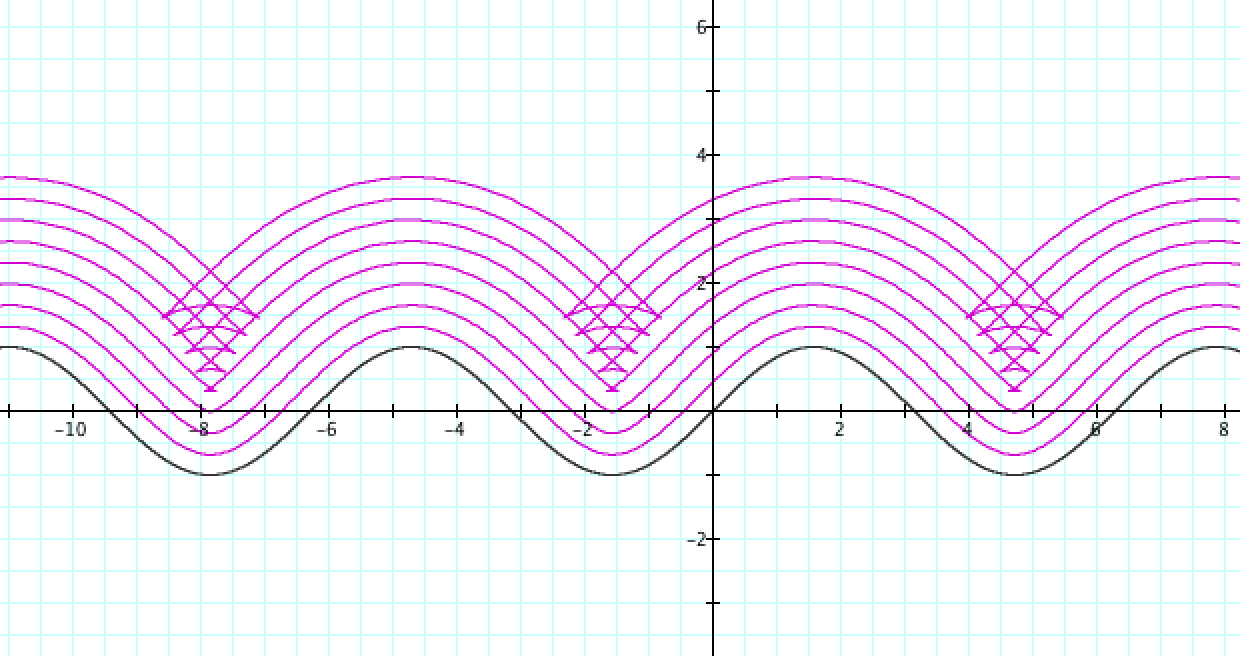
\includegraphics[width=\fw]{img/13-app/04.png}
  \caption{Caption}
\end{figure}

Consider on the other hand using a 3D printing machine to make a little plastic version of the function $y = sin(x)$. Make it perfectly exacting in shape but incredibly thin, almost wire thin. Now imagine walking to a perfectly still body of water (maybe a bath tub) and dropping the y=sin(x) shaped piece into the water horizontally so it all hits the surface at the exact same time. Can you guess what shape the resultant wave will be as it drifts away from $y = sin(x)$? Why it will perfectly resemble an $N$-Units Away Curve for that function!

I found this utterly fascinating and am very much so hoping to someday perform this exact experiment. I hope to film the whole thing with a nice high-speed camera and take a careful look at real world $N$-Units Away Curves!! How profoundly interesting. I didn't use to have any idea that these theoretical math constructions of mine had a role in the physical reality around us. To be honest, my question about said bath-tub $y = sin(x)$ wave experiment is the following: When the wave collapses upon itself at the crunch spots, probably one of two things will occur. Either we’ll see perfect nice little divot triangles form, exactly as in $N$-Units Away Theory, or we’ll see the water right in that area respond chaotically with turbulence instead. It’s very much so a question open for debate! In the real world, when you spot an $N$-Unit Away Curve, do the crunch spots create divot triangles or turbulence?

I leave that for my reader as a mystery for another day.
